\section{Geometric factor} \label{sec:geometric factor}

The flux of vertical muons whose momentum is greater than $\SI{1}{GeV/c}$ at sea level is $ I_0 \approx 70 \ \si{m^{-2}} \si{s^{-1}} \si{sr^{-1}}$ (see Section \ref{sec:introduction}) but this value refers to a single detector. However, the next working conditions require that the three scintillators to be employed in a coincidence state, forming a particle telescope \cite{Sullivan}, hence it is natural to expect a decrease in the radiation intensity detected, with respect to the nominal one. It is possible to estimate the intensity of radiation $I_0$ given the coincidence counting rate and the parameters (e.g. detectors dimensions) of our configuration. Since the calculus that follows has been done for an ideal telescope (i.e. the detection efficiency is $1$ for particles in a given energy range and $0$ otherwise), some assumption have been made: 
\begin{enumerate}
	\item Incident particles have rectilinear trajectories.
	\item The surface of the detectors considered has no thickness.
\end{enumerate}
The former can be reasonably accepted because in this experiment the particles that interact with the detectors are muons with a mean energy of $\sim \SI{4}{GeV}$ (see Section \ref{sec:introduction}). Nevertheless, the latter plays an important role since thickness is not negligible. So a Monte Carlo simulation has been performed to analyze if these assumptions are somewhat acceptable.\\
\indent If we consider an isotropic radiation $I=I_0$, the proportionality coefficient between the intensity $I$ and the coincidence rate $C$ is the \emph{geometric factor} $G$ of the telescope: $I\equiv I_0 = C/G$. Nevertheless, in this specific case the intensity of the particles distribution is not isotropic: $I = I_0\cdot \cos^2\theta$ \cite{PDG}. Therefore, a correction is needed when evaluating the geometric factor. However, in both cases the geometric factor has the unit of $\left[ \si{\meter}^{2}\cdot \si{\steradian}\right] $ and it is clear that this quantity represents the geometric acceptance of the particle telescope.\\
This value can be derived analytically for certain configurations \cite{Thomas} both for an isotropic and a $\cos^2\theta$-distributed intensity. In our case we have three rectangular scintillators one over the other but only the position and the dimensions of the first and the third detector affect the estimation of the geometrical factor. This assumption is justified due to the fact that the middle scintillator does not change the field of view of the telescope.
\begin{figure}[!htp]
	\centering
	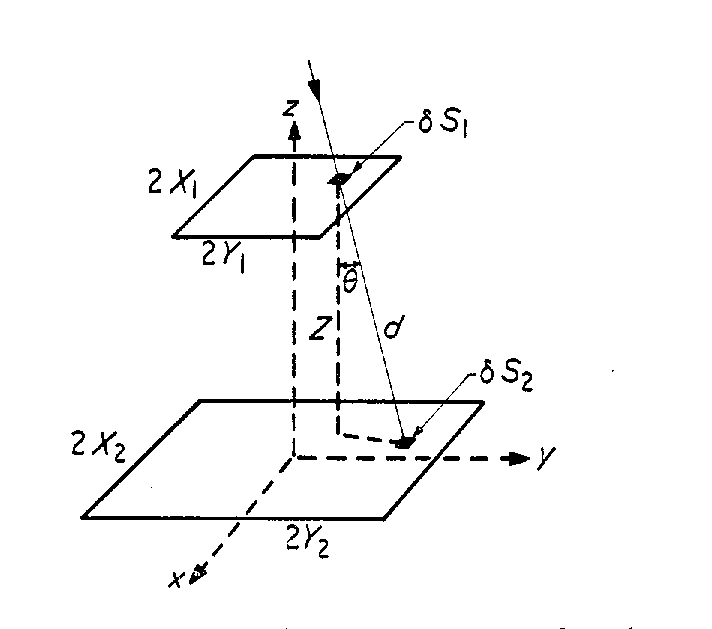
\includegraphics[height=5cm]{Thomas}
	\caption{Scheme of a particle telescope with two rectangular detectors.}
	\label{fig:Thomas}
\end{figure}
Referring to Figure \ref{fig:Thomas}, if we consider a telescope made of two rectangular detectors with sides $(2X_1,2Y_1)$ and $(2X_2,2Y_2)$ and a separation between them equal to $Z$, it is possible to obtain the explicit formula of the geometric factor\footnote{Considering a $\cos^2\theta$ distribution.}:
\begin{align}\label{eq:Thomas}
	G & = \frac{Z^2 + 2\left( X_1+X_2\right) ^2}{2\left[ Z^2 + \left( X_1+X_2\right)^2 \right] ^{\frac{1}{2}}} \cdot \left[ \left(Y_1+Y_2\right)\arctan\frac{Y_1+Y_2}{\left[ Z^2 + \left( X_1+X_2\right)^2 \right]^{\frac{1}{2}}} \right. \nonumber \\
	& \qquad \qquad \qquad \qquad \left. - \left(Y_2-Y_1\right)\arctan\frac{Y_2-Y_1}{\left[ Z^2 + \left( X_1+X_2\right)^2 \right]^{\frac{1}{2}}}\right] \nonumber \\
	%
	%Second term
	%
	&  - \frac{Z^2 + 2\left( X_2-X_1\right) ^2}{2\left[ Z^2 + \left( X_2-X_1\right)^2 \right] ^{\frac{1}{2}}} \cdot \left[ 	\left(Y_1+Y_2\right)\arctan\frac{Y_1+Y_2}{\left[ Z^2 + \left( X_2-X_1\right)^2 \right]^{\frac{1}{2}}} \right. \nonumber \\
	& \qquad \qquad \qquad \qquad \left. - \left(Y_2-Y_1\right)\arctan\frac{Y_2-Y_1}{\left[ Z^2 + \left( X_2-X_1\right)^2 \right]^{\frac{1}{2}}}\right] \nonumber \\
	%
	%Third term
	%
	& + \frac{Z^2 + 2\left( Y_1+Y_2\right) ^2}{2\left[ Z^2 + \left( Y_1+Y_2\right)^2 \right] ^{\frac{1}{2}}} \cdot \left[ \left(X_1+X_2\right)\arctan\frac{X_1+X_2}{\left[ Z^2 + \left( Y_1+Y_2\right)^2 \right]^{\frac{1}{2}}} \right. \nonumber \\
	& \qquad \qquad \qquad \qquad \left. - \left(X_2-X_1\right)\arctan\frac{X_2-X_1}{\left[ Z^2 + \left( Y_1+Y_2\right)^2 \right]^{\frac{1}{2}}}\right] \nonumber \\
	%
	%Fourth term
	%
	&  - \frac{Z^2 + 2\left( Y_2-Y_1\right) ^2}{2\left[ Z^2 + \left( Y_2-Y_1\right)^2 \right] ^{\frac{1}{2}}} \cdot \left[ \left(X_1+X_2\right)\arctan\frac{X_1+X_2}{\left[ Z^2 + \left( Y_2-Y_1\right)^2 \right]^{\frac{1}{2}}} \right. \nonumber \\
	& \qquad \qquad \qquad \qquad \left. - \left(X_2-X_1\right)\arctan\frac{X_2-X_1}{\left[ Z^2 + \left( Y_2-Y_1\right)^2 \right]^{\frac{1}{2}}}\right]
\end{align}
Since all of the three scintillators have the same width and length: $X_1 = X_2 = X$ and $Y_1 = Y_2 = Y$. Hence, it is clear that
\begin{equation}
	\begin{cases}\label{eq:condG_simplified}
		X_1 + X_2 = 2X \\
		Y_1 + Y_2 = 2Y \\
		X_2 - X_1 = 0 \\
		Y_2 - Y_1 = 0
	\end{cases}
\end{equation}
and thus it is possible to simplify \eqref{eq:Thomas} obtaining
\begin{align}\label{eq:Thomas_simplified}
	G & = \frac{Z^2 + 8X^2}{2\left( Z^2 + 4X^2 \right) ^{\frac{1}{2}}} \cdot \left[ 2Y\arctan\frac{2Y}{\left( Z^2 + 4X^2 \right)^{\frac{1}{2}}} \right]
	%
	%Second term
	%
	- \frac{Z}{2} \cdot \left( 2Y\arctan\frac{2Y}{Z} \right) \nonumber \\
	%
	%Third term
	%
	& + \frac{Z^2 + 8Y^2}{2\left( Z^2 + 4Y^2 \right) ^{\frac{1}{2}}} \cdot \left[ 2X\arctan\frac{2X}{\left( Z^2 + 4Y^2 \right)^{\frac{1}{2}}} \right]
	%
	%Fourth term
	%
	- \frac{Z}{2} \cdot \left( 2X\arctan\frac{2X}{Z} \right)
\end{align}
Using the coincidence counting rate `$C$'\footnote{It has been estimated as the double coincidences mean value.} given by the upper and the lower scintillators and the geometric factor calculated thanks to \eqref{eq:Thomas_simplified}, we can evaluate the intensity of the particles flux detected. In particular the intensity has been estimated as in \eqref{eq:intensity} where not only the coincidence rate and the geometric factor are present but also the efficiency of our telescope has been taken into account.
\begin{equation}\label{eq:intensity}
	I = \frac{C}{G\cdot\varepsilon_1 \varepsilon_2} \equiv \frac{C}{G\cdot\varepsilon_t}
\end{equation}
where $\varepsilon_1, \varepsilon_2$ are the efficiencies of the upper and lower detector and $\varepsilon_{t} = \varepsilon_1 \varepsilon_2$ is the overall efficiency of the particle telescope.
\begin{figure}[!htp]
	\centering
	\begin{subfigure}{.3\textwidth}
		\centering
		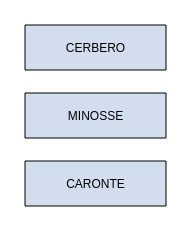
\includegraphics[width=.7\textwidth]{layout1}
		\caption{Layout 1}\label{subfig:l1}
	\end{subfigure}\hfill
	\begin{subfigure}{.3\textwidth}
		\centering
		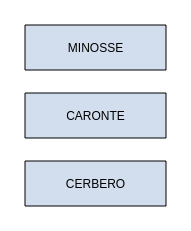
\includegraphics[width=.7\textwidth]{layout3}
		\caption{Layout 2}\label{subfig:l2}
	\end{subfigure}\hfill
	\begin{subfigure}{.3\textwidth}
		\centering
		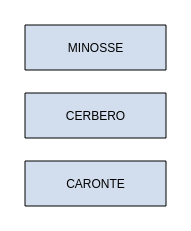
\includegraphics[width=.7\textwidth]{layout2}
		\caption{Layout 3}\label{subfig:l3}
	\end{subfigure}
	\caption{All the possible configurations with three detectors. Note that the exchange of the external scintillators does not affect the geometric factor.}
	\label{fig:telescopes_layout}
\end{figure}
Results (with respect to Figure \ref{fig:telescopes_layout}) are reported in Table \ref{tab:intensities},
\begin{table}[!htp]
	\centering
	\begin{tabular}{r|ccc}
		\toprule
		& $C \ \left[ \si{\second}^{-1}\right] $ & $G \ \left[ \si{\meter}^{2}\cdot \si{\steradian}\right] $ & $I \ \left[ \si{\meter}^{-2} \cdot \si{\second}^{-1} \cdot \si{\steradian}^{-1}\right] $\\
		\midrule
		Layout 1 & $22.5$ & $0.3112$ & $73.17$\\
		Layout 2 & $18.6$ & $0.3112$ & $60.32$\\ 
		Layout 3 & $18.7$ & $0.2602$ & $72.90$\\
		\bottomrule
	\end{tabular}
	\caption{Incident particles intensities for the three possible configurations.}
	\label{tab:intensities}
\end{table}
where we can see that the $G$ factor, as well as the distance\footnote{The dead layer of the detectors has been taken into account during the estimation of the distance.} $Z$ between the upper scintillator and the lower one (see Table \ref{tab:set-up}), is the same for Layout 1 and 2, but different from the third one.
\begin{table}[!htp]
	\centering
	\begin{tabular}{cc}
		\toprule
		Variable & Value ($\si{\meter}$)\\
		\midrule
		$2X_1$ & $0.800 \pm 0.001$\\
		$2Y_1$ & $0.300 \pm 0.001$\\
		$2X_2$ & $0.800 \pm 0.001$\\
		$2Y_2$ & $0.300 \pm 0.001$\\
		$Z$ & $0.080 \pm 0.005$\\
		\bottomrule
		&\\
		\multicolumn{2}{c}{\footnotesize (a) \emph{Layout 1}}
	\end{tabular}\hfill
	\begin{tabular}{cc}
		\toprule
		Variable & Value ($\si{\meter}$)\\
		\midrule
		$2X_1$ & $0.800 \pm 0.001$\\
		$2Y_1$ & $0.300 \pm 0.001$\\
		$2X_2$ & $0.800 \pm 0.001$\\
		$2Y_2$ & $0.300 \pm 0.001$\\
		$Z$ & $0.080 \pm 0.005$\\
		\bottomrule
		&\\
		\multicolumn{2}{c}{\footnotesize (a) \emph{Layout 2}}
	\end{tabular}\hfill
	\begin{tabular}{cc}
		\toprule
		Variable & Value ($\si{\meter}$)\\
		\midrule
		$2X_1$ & $0.800 \pm 0.001$\\
		$2Y_1$ & $0.300 \pm 0.001$\\
		$2X_2$ & $0.800 \pm 0.001$\\
		$2Y_2$ & $0.300 \pm 0.001$\\
		$Z$ & $0.150 \pm 0.005$\\
		\bottomrule
		&\\
		\multicolumn{2}{c}{\footnotesize (a) \emph{Layout 3}}
	\end{tabular}
	\caption{Geometrical parameters of the detectors setup. $Z$ represents the distance between the upper and the lower detectors while the couple $\left(2X_{1/2}, 2Y_{1/2}\right)$ are the length and width, respectively, of the scintillators.}
	\label{tab:set-up}
\end{table}
Now it is possible to propagate the errors both in \eqref{eq:Thomas_simplified} and in the evaluation of the intensities \eqref{eq:intensity}.\\
The errors propagation formula for a general function $f = f\left( x_1, x_2, \dots, x_n\right)$ is
\begin{equation}\label{eq:error_propagation}
	\sigma_f = \sqrt{\sum_{i = 1}^{n}\left( \frac{\partial f}{\partial x_i}\cdot \sigma_{x_i}\right)^2 + \underbrace{2\sum_{i\ne j}\frac{\partial f}{\partial x_i}\frac{\partial f}{\partial x_j}\cdot \sigma_{x_i x_j}}_{C_{x_i x_j}}}
\end{equation}
Since the variables $X,Y,Z$ are not correlated we can neglect covariances when computing the uncertainty on $G$ \eqref{eq:Thomas_simplified}. However, in \eqref{eq:intensity} there is an obvious correlation between $C$ and $\varepsilon_t$ so $C_{x_i x_j}$ has to be taken into account. Despite it is not possible to evaluate this quantity we can do some general considerations: first of all, it is clear that the correlation between the efficiencies and the counting rate is positive. As a consequence, if we underestimate $\varepsilon_1$ or $\varepsilon_2$ we will underestimate $C$, i.e. the covariance term is a positive quantity. Due to the fact that the derivatives of the intensities with respect to $C$ and $\varepsilon_t$ have opposite signs, it follows that neglecting the covariance term leads to an overestimation of the error.
% In addition it is possible to say that the covariance is a positive quantity due to the fact that the derivatives of the intensity with respect to $C$ and $\varepsilon_{t}$ are positive too. It follows that neglecting the covariance leads to an underestimation of the error.\\

\begin{table}[!htp]
	\centering
	\begin{tabular}{r|ccc}
		\toprule
		& $C \ \left[ \si{\second}^{-1}\right] $ & $G \ \left[ \si{\meter}^{2}\cdot \si{\steradian}\right] $ & $I \ \left[ \si{\meter}^{-2} \cdot \si{\second}^{-1} \cdot \si{\steradian}^{-1}\right] $\\
		\midrule
		Layout 1 & $22.5\pm0.6$ & $0.3112\pm0.0043$ & $73.17\pm2.25$\\
		Layout 2 & $18.6\pm2.5$ & $0.3112\pm0.0043$ & $60.32\pm8.01$\\ 
		Layout 3 & $18.7\pm0.4$ & $0.2602\pm0.0038$ & $72.90\pm1.79$\\
		\bottomrule
	\end{tabular}
	\caption{Incident particles intensities for the three possible configuration, errors estimation included.}
	\label{tab:Thomas_results}
\end{table}
\indent In order to evaluate if our results (presented in Table \ref{tab:Thomas_results}) are in accordance with the expected value of $I_0 = 70 \ \si{\meter}^{-2} \cdot \si{\second}^{-1} \cdot \si{\steradian}^{-1} $, we performed a $t$-test.
\begin{equation}\label{eq:zTest}
	t = \frac{\left| I_{meas} - I_0\right|}{\sigma_{I_{meas}}} 
\end{equation}
After that it is possible to estimate the \emph{p-value} and to conclude that the intensities found for the three layouts are acceptable assuming a significance level of $\alpha = 0.05$. This fact confirms our hypothesis of detecting predominantly muons. Nevertheless, as it is possible to see in Table \ref{tab:accordance}, the agreement percentage is low, probably due to the strict assumptions made while deriving the equation \eqref{eq:Thomas_simplified}.\\
To test this hypothesis in Section \ref{sec:aligned} we performed a Monte Carlo simulation as mentioned at the beginning of this section.
\begin{table}[!htp]
	\centering
	\begin{tabular}{r|cc}
		\toprule
		& \emph{t-value} & \emph{p-value} \\
		\midrule
		Layout 1 & $1.41$ & $0.1585$ \\
		Layout 2 & $1.21$ & $0.2263$ \\ 
		Layout 3 & $1.62$ & $0.1052$ \\
		\bottomrule
	\end{tabular}
	\caption{Accordance between the estimated and expected muons intensity.}
	\label{tab:accordance}
\end{table}
